% Diagrama: Escala Garibelt — espectro de 4 bandas
% Usado en: 5-Analisis-Red-Actual/5-6-Clasificacion-Garibelt/5-6-2-Clasificacion.tex
% fig:escala-garibelt-barra
%
% Barra horizontal [0,1] con 4 zonas de color, etiquetas internas,
% valores de corte en la parte inferior y descripción de cada banda.
% Ancho diseñado para \textwidth (≈ 13 cm con márgenes de tesis).

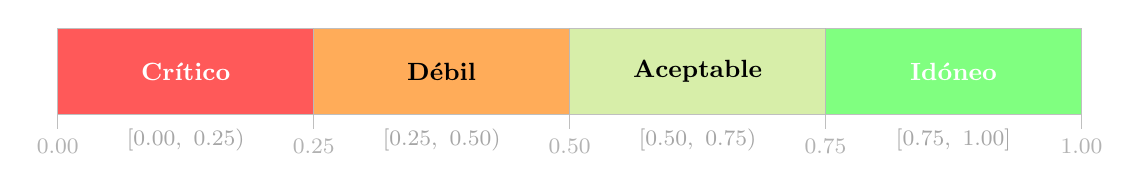
\begin{tikzpicture}

% ================================================================
%  Barra principal — ancho 13 cm, alto 1.1 cm
%  Bandas: 0–3.25 / 3.25–6.50 / 6.50–9.75 / 9.75–13.00
% ================================================================
\fill[red!65]             (0.00, 0) rectangle ( 3.25, 1.10);
\fill[orange!65]          (3.25, 0) rectangle ( 6.50, 1.10);
\fill[yellow!55!green!35] (6.50, 0) rectangle ( 9.75, 1.10);
\fill[green!50]           (9.75, 0) rectangle (13.00, 1.10);
\draw[gray!50, thin]      (0.00, 0) rectangle (13.00, 1.10);
\draw[gray!55, thin] (3.25, 0) -- (3.25, 1.10);
\draw[gray!55, thin] (6.50, 0) -- (6.50, 1.10);
\draw[gray!55, thin] (9.75, 0) -- (9.75, 1.10);

% Etiquetas de banda (centradas en cada zona)
\node[font=\small\bfseries, white]           at (1.625, 0.55) {Crítico};
\node[font=\small\bfseries]                  at (4.875, 0.55) {Débil};
\node[font=\small\bfseries]                  at (8.125, 0.55) {Aceptable};
\node[font=\small\bfseries, white]           at (11.375, 0.55) {Idóneo};

% Rangos numéricos debajo de cada banda
\node[font=\footnotesize, color=gray!70, anchor=north] at (1.625, -0.05)
    {$[0.00,\ 0.25)$};
\node[font=\footnotesize, color=gray!70, anchor=north] at (4.875, -0.05)
    {$[0.25,\ 0.50)$};
\node[font=\footnotesize, color=gray!70, anchor=north] at (8.125, -0.05)
    {$[0.50,\ 0.75)$};
\node[font=\footnotesize, color=gray!70, anchor=north] at (11.375, -0.05)
    {$[0.75,\ 1.00]$};

% Ticks en los puntos de corte
\foreach \xval in {0.00, 3.25, 6.50, 9.75, 13.00}{
    \draw[gray!50] (\xval, 0) -- (\xval, -0.18);
}
\node[font=\footnotesize, color=gray!60, anchor=north] at (0.00,  -0.18) {$0.00$};
\node[font=\footnotesize, color=gray!60, anchor=north] at (3.25,  -0.18) {$0.25$};
\node[font=\footnotesize, color=gray!60, anchor=north] at (6.50,  -0.18) {$0.50$};
\node[font=\footnotesize, color=gray!60, anchor=north] at (9.75,  -0.18) {$0.75$};
\node[font=\footnotesize, color=gray!60, anchor=north] at (13.00, -0.18) {$1.00$};

\end{tikzpicture}
